\section{DuoHash: the new version of MISSH}
\label{sec:DuoHash}

The final improvement of the \acs{MISSH} tool took shape with the introduction of a new strategy to calculate the hashing of nucleotide sequences, significantly reducing the calculation time and increasing the overall efficiency of the process. The original hash function from which the optimisation started is the rolling hash function, the pseudo-code of which is shown in Algorithm~\ref{alg:duohash-original-rolling-hash}.

\begin{algorithm}[!ht]
	\caption{Rolling Hash function}
	\label{alg:duohash-original-rolling-hash}
	
	$\mathrm{values} \gets \{ \texttt{0x3C8BFBB395C60474}, \texttt{0x3193C18562A02B4C}, \allowbreak\texttt{0x20323ED082572324}, \texttt{0x295549F54BE24456} \}$\;
	
	\SetKwFunction{FrollingHash}{getHashes}
	\Fn{\FrollingHash{$x$, $Q$, $i$}}{
		$forward \gets 0$\;
		$reverse \gets 0$\;
		\ForEach{$k \in Q$}{
			$index \gets \texttt{char\_to\_int}(x[i + k])$\tcp*{defined at Page~\pageref{alg:original_encoding_function}}
			$forward \gets forward \oplus \rol^{|Q| - 1 - k} \mathrm{values}[index]$\;
			$reverse \gets reverse \oplus \rol^{k} \mathrm{values}[|\mathrm{values}| - 1 - index]$\;
		}
		\KwRet{$\langle forward, reverse \rangle$}\;
	}
\end{algorithm}

The DuoHash approach exploits initial encoding\footnote{In the DuoHash tool, what was called "encoding" in previous versions was called "hashing".} and a structure called \verb|Hash| that contains the variables for forward and reverse hashing. The basic idea behind the new algorithm is the use of tables with pre-calculated hashes to speed up the hash calculation process. Instead of calculating the hash for each nucleotide base at runtime, look-up tables are used that contain pre-calculated values for all possible combinations of four nitrogen bases. This approach drastically reduces the number of operations required.

\begin{example}
	To better explain the concept, let us consider an example of look-up tables. 
	\begin{center}
		\begin{tabular}{c c c}
			\textbf{sequence} & \textbf{encoding} & \textbf{hashing} \\
			\toprule
			\verb|AAAA| & \verb|00000000| & \verb|0x53EC3F8647623EED| \\
			\verb|CAAA| & \verb|00000001| & \verb|0x3B2DEE31FC53472D| \\
			\verb|GAAA| & \verb|00000010| & \verb|0xB622149EFBEB046D| \\
			\verb|TAAA| & \verb|00000011| & \verb|0xFD19ADB0B6403FFD| \\
			\verb|ACAA| & \verb|00000100| & \verb|0x678CD75D9AFA820D| \\
			\verb|...| & \verb|...| & \verb|...| \\
			\verb|TTTT| & \verb|11111111| & \verb|0x9400B260ACBDFF13| \\
			\bottomrule
		\end{tabular}
	\end{center}
	
	Given the nucleotide sequence $x = \texttt{AGGCCCACTGGAAGTTGTAGCCACCG}$ and the spaced seed \verb|11110111011100111011101111| defined as $Q = \{ 0, 1, 2, \allowbreak3, 5, 6, 7, 9, 10, 11, 14, 15, 16, 18, 19, 20, 22, 23, 24, 25 \}$, the $Q$-gram $x[0 + Q]$ is calculated as follows:
	\begin{center}
		\begin{tabular}{r || l}
			$x$ & \texttt{AGGCCCACTGGAAGTTGTAGCCACCG} \\
			$Q$ & \texttt{11110111011100111011101111} \\
			$x[0 + Q]$ & \texttt{AGGC\ CAC\ GGA\ \ TTG\ AGC\ ACCG} \\
		\end{tabular}
	\end{center}
	
	The resulting $Q$-gram is $x[0 + Q] = \texttt{AGGCCACGGATTGAGCACCG}$. Its encoding, in accordance with \acs{MISSH} and earlier versions, is \[ h(x[0 + Q]) = \texttt{1001010001100010111100101001000101101000} \]
	
	A total of $k = 5$ groups of 8 bits (corresponding to the encoding of 4 bases) are counted. Each of these groups is used as an index to access the pre-calculated hash tables:
	\begin{center}
		\begin{tabular}{r c c}
			\textbf{i} & \textbf{encoding} & \textbf{hashing} \\
			\toprule
			0 & \verb|01101000| & \verb|0x15609AFAC162C235| \\
			1 & \verb|10010001| & \verb|0x3DA45F3F050E3E0D| \\
			2 & \verb|11110010| & \verb|0x8841C2559987C40B| \\
			3 & \verb|01100010| & \verb|0x8249A46E23AF65F5| \\
			4 & \verb|10010100| & \verb|0x6105665363A7FB2D| \\
			\bottomrule
		\end{tabular}
	\end{center}
	
	The hashing value is then calculated using the following formula: \[ \text{hashing} = \bigoplus_{i = 0}^{k - 1} \rol^{4 \cdot (k - i - 1)} \text{look-up}[i] \] 
	In the example case, hashing takes the value \begin{align*}
		\text{hashing} &= \texttt{0x9AFAC162C2351560} \oplus \texttt{0x45F3F050E3E0D3DA} \oplus {} \\
		&\quad {} \oplus \texttt{0x41C2559987C40B88} \oplus \texttt{0x249A46E23AF65F58} \oplus {} \\
		&\quad {} \oplus \texttt{0x6105665363A7FB2D} \\
		&= \texttt{0xDB54441AFF406947} 
	\end{align*}
	
	Figure~\ref{fig:lookup-table} may help in understanding the process.
\end{example}

\begin{figure}[!ht]
	\centering
	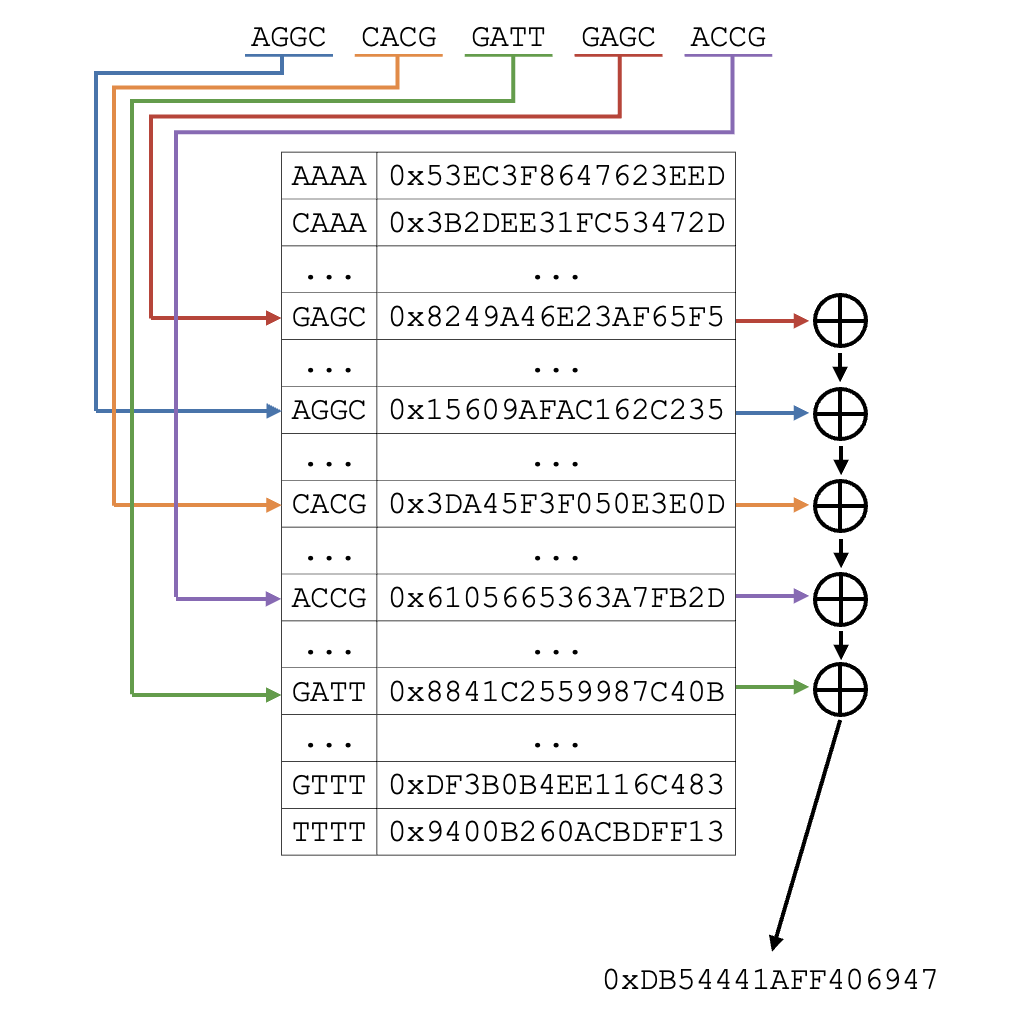
\includegraphics[width=0.85\linewidth]{images/lookup-table}
	\caption[Schematic procedure for using look-up tables.]{Schematic and visual procedure for using look-up tables to calculate the hashing value of the $Q$-gram \texttt{AGGCCACGGATTGAGCACCG}.}
	\label{fig:lookup-table}
\end{figure}

To better handle forward and reverse hashing, and cases where the last group of 4 nitrogen bases is not completely filled, there are 8 look-up tables:
\begin{itemize}
	\item \verb|e4_to_fHash| and \verb|e4_to_rHash| for handling complete groups of all 4 bases;
	\item \verb|e3_to_fHash| and \verb|e3_to_rHash| for the management of groups composed of 3 bases;
	\item \verb|e2_to_fHash| and \verb|e2_to_rHash| for the management of groups consisting of 2 bases;
	\item \verb|e1_to_fHash| and \verb|e1_to_rHash| for the management of groups with only 1 base.
\end{itemize}

Each table used to manage groups composed of $k$ nitrogen bases contains $4^k$ values. For each of these values, the corresponding shifts are also pre-calculated, avoiding shift operations at runtime. Taking into account that spaced seeds with a maximum weight of 32 are allowed, and that the values in the look-up tables are in groups of 4 nitrogenous bases, the possible shifts are 8. Considering that each table contains $4^k$ values, that for each value the corresponding 8 shifts are also pre-calculated, and that each value is a 64-bit integer (8 Bytes), each table requires memory space equal to $4^{k + 3} \text{ Bytes}$. In total, the look-up tables occupy a total space of $21.25 \text{ kBytes}$\footnote{$1 \text{ Byte} = 8 \text{ bits}$; $1 \text{ kByte} = 1024 \text{ Bytes}$.}. With modern memory capacities, the space required to handle the 8 look-up tables is acceptable. The Algorithm~\ref{alg:DuoHash-lookup-table} describes how the look-up tables are pre-calculated.

\begin{algorithm}[!ht]
	\caption{DuoHash: look-up tables}
	\label{alg:DuoHash-lookup-table}
	
	$\mathrm{values} \gets \{ \texttt{0x3C8BFBB395C60474}, \texttt{0x3193C18562A02B4C}, \allowbreak\texttt{0x20323ED082572324}, \texttt{0x295549F54BE24456} \}$\;
	
	\SetKwFunction{FlookupTable}{lookupTable}
	\Fn{\FlookupTable{$k$}}{
		\For{$i \gets 0$ \KwTo $4^k - 1$}{
			$\mathrm{e}k\mathrm{\_to\_fHash}[i][0] \gets 0$\;
			$\mathrm{e}k\mathrm{\_to\_rHash}[i][0] \gets 0$\;
			
			\tcc{For loop to prepare primary hashing values}
			\For{$j \gets 0$ \KwTo $k - 1$}{
				$index \gets (i >\!> 2j) \land \texttt{0b11}$\;
				$\mathrm{e}k\mathrm{\_to\_fHash}[i][0] \gets \mathrm{e}k\mathrm{\_to\_fHash}[i][0] \oplus \rol^{k - j - 1} \mathrm{values}[index]$\;
				$\mathrm{e}k\mathrm{\_to\_rHash}[i][0] \gets \mathrm{e}k\mathrm{\_to\_rHash}[i][0] \oplus \rol^{j} \mathrm{values}[|\mathrm{values}| - 1 - index]$\;
			}
			
			\tcc{For loop to populate the shifts table}
			\For{$j \gets 0$ \KwTo $8 - 1$}{
				$\mathrm{e}k\mathrm{\_to\_fHash}[i][j] \gets \rol^{4j} \mathrm{e}k\mathrm{\_to\_fHash}[i][0]$\;
				$\mathrm{e}k\mathrm{\_to\_rHash}[i][j] \gets \rol^{4j} \mathrm{e}k\mathrm{\_to\_rHash}[i][0]$\;
			}
		}
		\KwRet{$\langle \mathrm{e}k\mathrm{\_to\_fHash}, \mathrm{e}k\mathrm{\_to\_rHash} \rangle$}\;
	}
\end{algorithm}




The starting point of the new algorithm is the production of only the encoding of the nucleotide sequence, i.e. what was called the hashing value in previous versions of the software. This encoding is stored within a structure called \verb|Hash|, which also contains two variables set for forward and reverse hashing. The latter are calculated only later, using the specially optimised \verb|getHashes| function. The function, as illustrated in the Algorithm~\ref{alg:DuoHash}, receives two parameters: the structure \verb|Hash| and the value $s(Q)$. The variable \verb|encoding| is temporarily broken down into bytes, each of which represents the encoding of 4 nitrogen bases. Using the byte value as an index, the function accesses a series of tables of pre-calculated values, as described in the previous section.

\begin{algorithm}[!ht]
	\caption{DuoHash: getHashes function}
	\label{alg:DuoHash}
	
	\SetKwFunction{FgetHashes}{getHashes}
	\Fn{\FgetHashes{$Hash$, $s(Q)$}}{
		$bytes \gets s(Q) / 4$\tcp*{$Hash = \langle encoding, forward, reverse \rangle$}
		\For{$i \gets 0$ \KwTo $bytes$}{
			$curr\_byte \gets i$-th byte of $encoding$\;
			$forward \gets forward \oplus \mathrm{e4\_to\_fHash}[curr\_byte][bytes - i - 1]$\;
			$reverse \gets reverse \oplus \mathrm{e4\_to\_rHash}[curr\_byte][i]$\;
		}
		
		\If{$s(Q) \bmod 4 \neq 0$}{
			$curr\_byte \gets bytes$-th byte of $encoding$\;
			$forward \gets \rol^{s(Q) \bmod 4} forward$\;
			
			\If{$s(Q) \bmod 4 = 3$}{
				$forward \gets forward \oplus \mathrm{e3\_to\_fHash}[curr\_byte][0]$\;
				$reverse \gets reverse \oplus \mathrm{e3\_to\_rHash}[curr\_byte][bytes]$\;
			}
			\ElseIf{$s(Q) \bmod 4 = 2$}{
				$forward \gets forward \oplus \mathrm{e2\_to\_fHash}[curr\_byte][0]$\;
				$reverse \gets reverse \oplus \mathrm{e2\_to\_rHash}[curr\_byte][bytes]$\;
			}
			\ElseIf{$s(Q) \bmod 4 = 1$}{
				$forward \gets forward \oplus \mathrm{e1\_to\_fHash}[curr\_byte][0]$\;
				$reverse \gets reverse \oplus \mathrm{e1\_to\_rHash}[curr\_byte][bytes]$\;
			}
		}
	}
\end{algorithm}

This solution was developed to address some of the limitations of the previous techniques used in \acs{MISSH}, which, although effective, had room for improvement in terms of computational efficiency. The new strategy is based on the idea of avoiding the repetitive calculation of the same values and instead exploiting a pre-computed look-up table, which drastically reduces the number of operations required to obtain the desired hashes. The \verb|getHashes| function was implemented to make the most of this optimisation, ensuring that the necessary values are always readily available without having to recalculate them each time. The approach taken also takes into account the need to handle variable-length sequences efficiently. Indeed, handling $s(Q) \bmod 4$ makes it possible to deal with cases where the length of the sequence is not an exact multiple of 4 nitrogenous bases. 

A further significant advantage of this implementation is the ease with which the hashing function can be modified. Thanks to the modular structure, it is possible to update the \verb|getHashes| function to switch from a rolling hash function to any other hashing function, without having to modify other parts of the code. This makes the tool extremely flexible and easily adaptable to new requirements or hashing algorithms, improving its longevity and usefulness. The possibility of easily changing the hashing function is made possible by the fact that the encoding, initially calculated by \acs{MISSH}, provides a robust and flexible basis on which different hashing strategies can be applied. The integration of this new hashing function with the other components of \acs{MISSH} required careful consideration of the overall architecture of the tool. The decision to initially produce only the forward encoding and to postpone the calculation of the forward and reverse hashes to a later stage was taken in order to maximise efficiency and reduce the initial computational load. This approach allows all the necessary encodings to be accumulated before proceeding with the calculation of the hashes, thus optimising the use of resources and improving the overall speed of the process. Furthermore, the choice of using a \verb|Hash| structure to contain both the encoding and the forward and reverse hashes made the code more modular and easier to maintain. This structure makes it possible to isolate the calculation of the hashes from other operations, facilitating debugging and eventual updating of the code. The \verb|getHashes| function has been designed to be highly efficient, minimising the number of operations required and making maximum use of the calculation capabilities of modern CPUs.

The innovative approach adopted in this new tool DuoHash represents a significant step forward compared to previously used techniques. The combination of an optimised data structure, the use of pre-computed look-up tables and the efficient management of remainders results in a significant improvement in performance, making the tool more competitive and suitable for handling large amounts of data with greater speed and accuracy. The benefits of this approach will be further explored in the following chapters, where the results of performance tests and comparisons with other tools will be presented, demonstrating the effectiveness and superiority of the new strategy adopted.
